

%Tex File: D:/R_projects/MScED_Dissertation/tex/tables/reduced.tex

\begin{table}[!htbp] \centering 
  \caption{Reduced Form Effects in No-First-Stage Samples} 
  \label{tab:reduced} 
\begin{threeparttable}
\begin{tabular}{@{\extracolsep{5pt}}lcccc} 
\\[-1.8ex]\hline 
\hline \\[-1.8ex] 
 & \multicolumn{2}{c}{Twins2$^{\dag}$} & \multicolumn{2}{c}{Boy12$^{\ddag}$} \\
 \cline{2-3} \cline{4-5} \\
 & Spacing $<$ 2 & No Schooling & Spacing $<$ 2 & No Schooling \\
\\[-1.8ex] & (1) & (2) & (3) & (4)\\ 
\hline \\[-1.8ex] 
\\[-2.0ex] \multicolumn{5}{@{} l}{\textbf{Panel A: First Stage}}
 \\
 \\[-1.5ex]
 No. of children & 0.266$^{*}$ & 0.101 & $-$0.0004 & 0.041 \\ 
  & (0.141) & (0.134) & (0.037) & (0.046) \\ 
  & & & & \\ 
\\[-1.83ex] 
 \hline \\[-1.83ex]
\\[-2.0ex] \multicolumn{5}{@{} l}{\textbf{Panel B: Reduced Form$^{\S}$}}
 \\
 \\[-1.5ex]
 Educational Attainment & 0.031 & 0.006 & 0.001 & 0.007 \\ 
  & (0.025) & (0.021) & (0.006) & (0.007) \\ 
  & & & & \\ 
 Left Behind & $-$0.131$^{*}$ & $-$0.067 & 0.013 & $-$0.026 \\ 
  & (0.070) & (0.067) & (0.018) & (0.020) \\ 
  & & & & \\ 
 Private School & 0.027 & $-$0.011$^{***}$ & 0.005 & 0.001 \\ 
  & (0.053) & (0.004) & (0.011) & (0.006) \\ 
  & & & & \\ 
 Mothers LFP & 0.033 & $-$0.052 & 0.034$^{**}$ & 0.005 \\ 
  & (0.065) & (0.067) & (0.015) & (0.020) \\ 
  & & & & \\ 
\hline \\[-1.8ex] 
 $ N $  & 3,489 & 3,022 & 2,869 & 2,381 \\
\hline 
\hline \\[-1.8ex] 
\end{tabular} 
\begin{tablenotes}
\footnotesize
\item \textit{Notes:} *** Significant at 1\%, ** Significant at 5\%, * Significant at 10\%. 
The same set of covariates as in \autoref{tab:main-res} were included in all regressions. Robust standard
errors in parentheses.
\\[-1.8ex]

$ \dag $ The subsamples are restricted to firstborns from families with at least three children.

$ \ddag $ Subsamples includes only firstborn boys.

$ \S $ In addition to the covariates used in \autoref{tab:main-res}, the reduced form regressions control for 
the number of children in the family.
\end{tablenotes}
\end{threeparttable}
\end{table} 




\pagebreak

\begin{figure}[p!]
\centering
\caption{\label{fig:heter1}Results of Generalized Random Forest Using Twins IV}
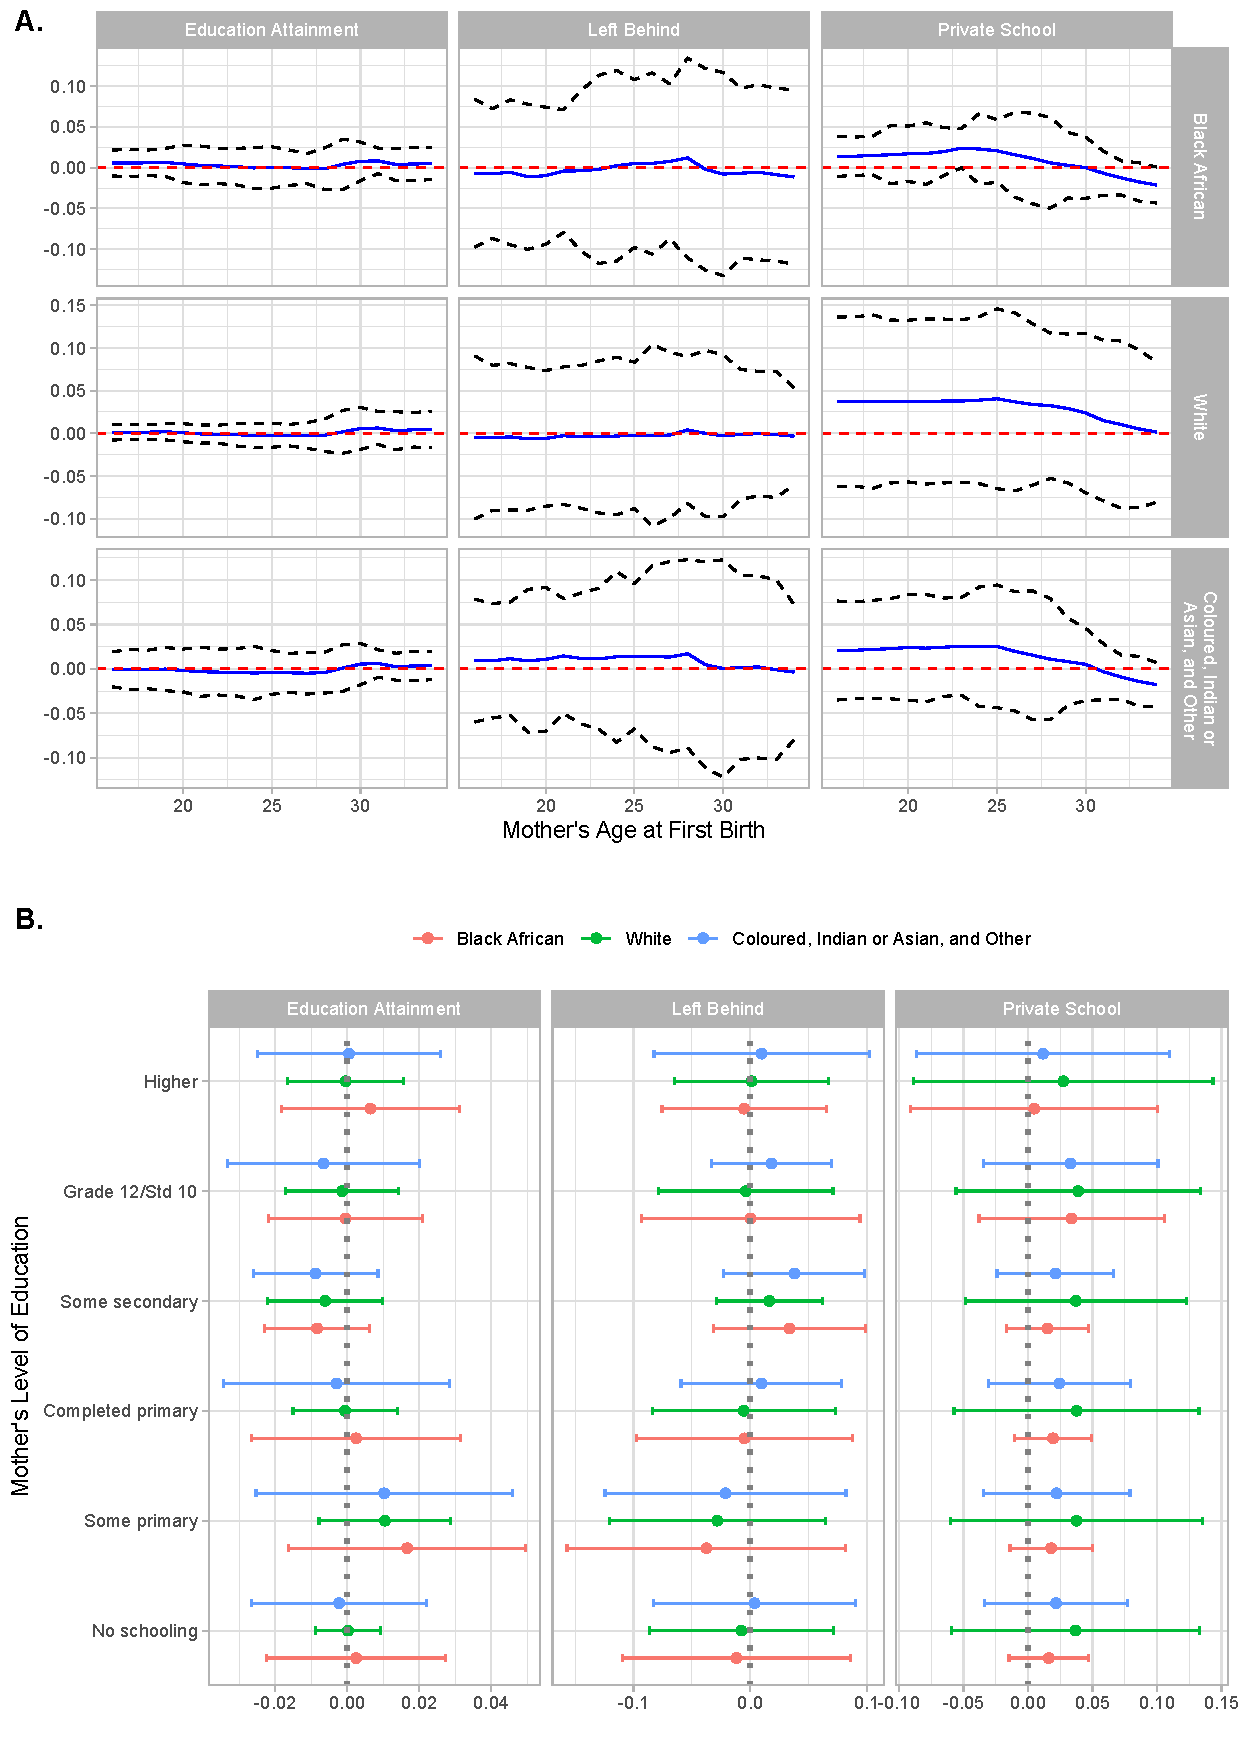
\includegraphics[width=\textwidth]{figures/heter1.pdf}
\fnote{\textit{Notes:} The above results are based on three forests, one forest for each outcome. Tuning results suggest the default values of the parameters as optimal for each forest. Each forest is based on 5000 trees. }
\end{figure}
\pagebreak

\begin{figure}[p!]
\centering
\caption{\label{fig:heter2}Results of Generalized Random Forest Using Same-Sex IV}
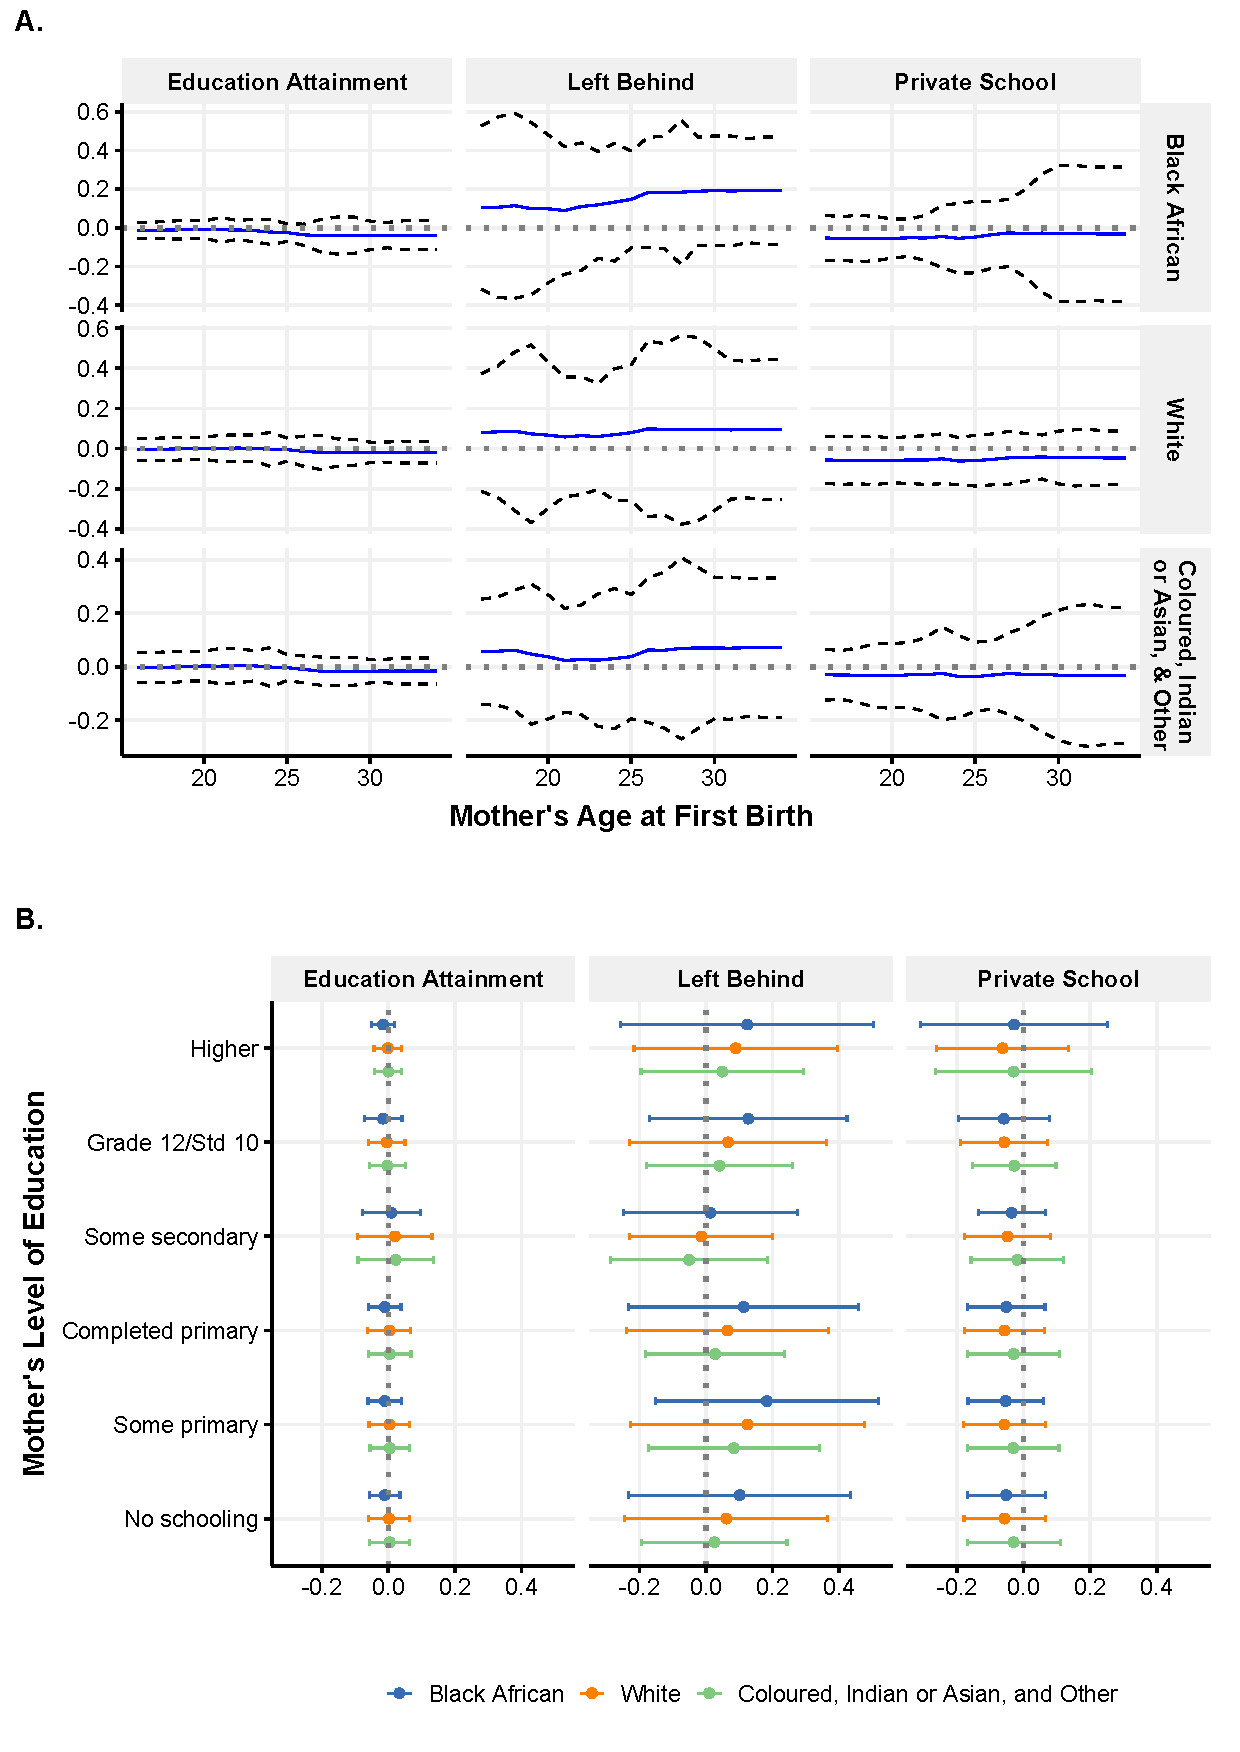
\includegraphics[width=\textwidth]{figures/heter2.pdf}
\fnote{\textit{Notes:} The above results are based on three forests, one forest for each outcome. The parameters supplied in training each forest were chosen by tuning based on cross-validation. Each forest is based on 5000 trees. }
\end{figure}
\pagebreak

\begin{figure}[ht]
\centering
\caption{\label{fig:02}Unconditional First-Stages and 95\% Confidence Intervals for Different Family Sizes}
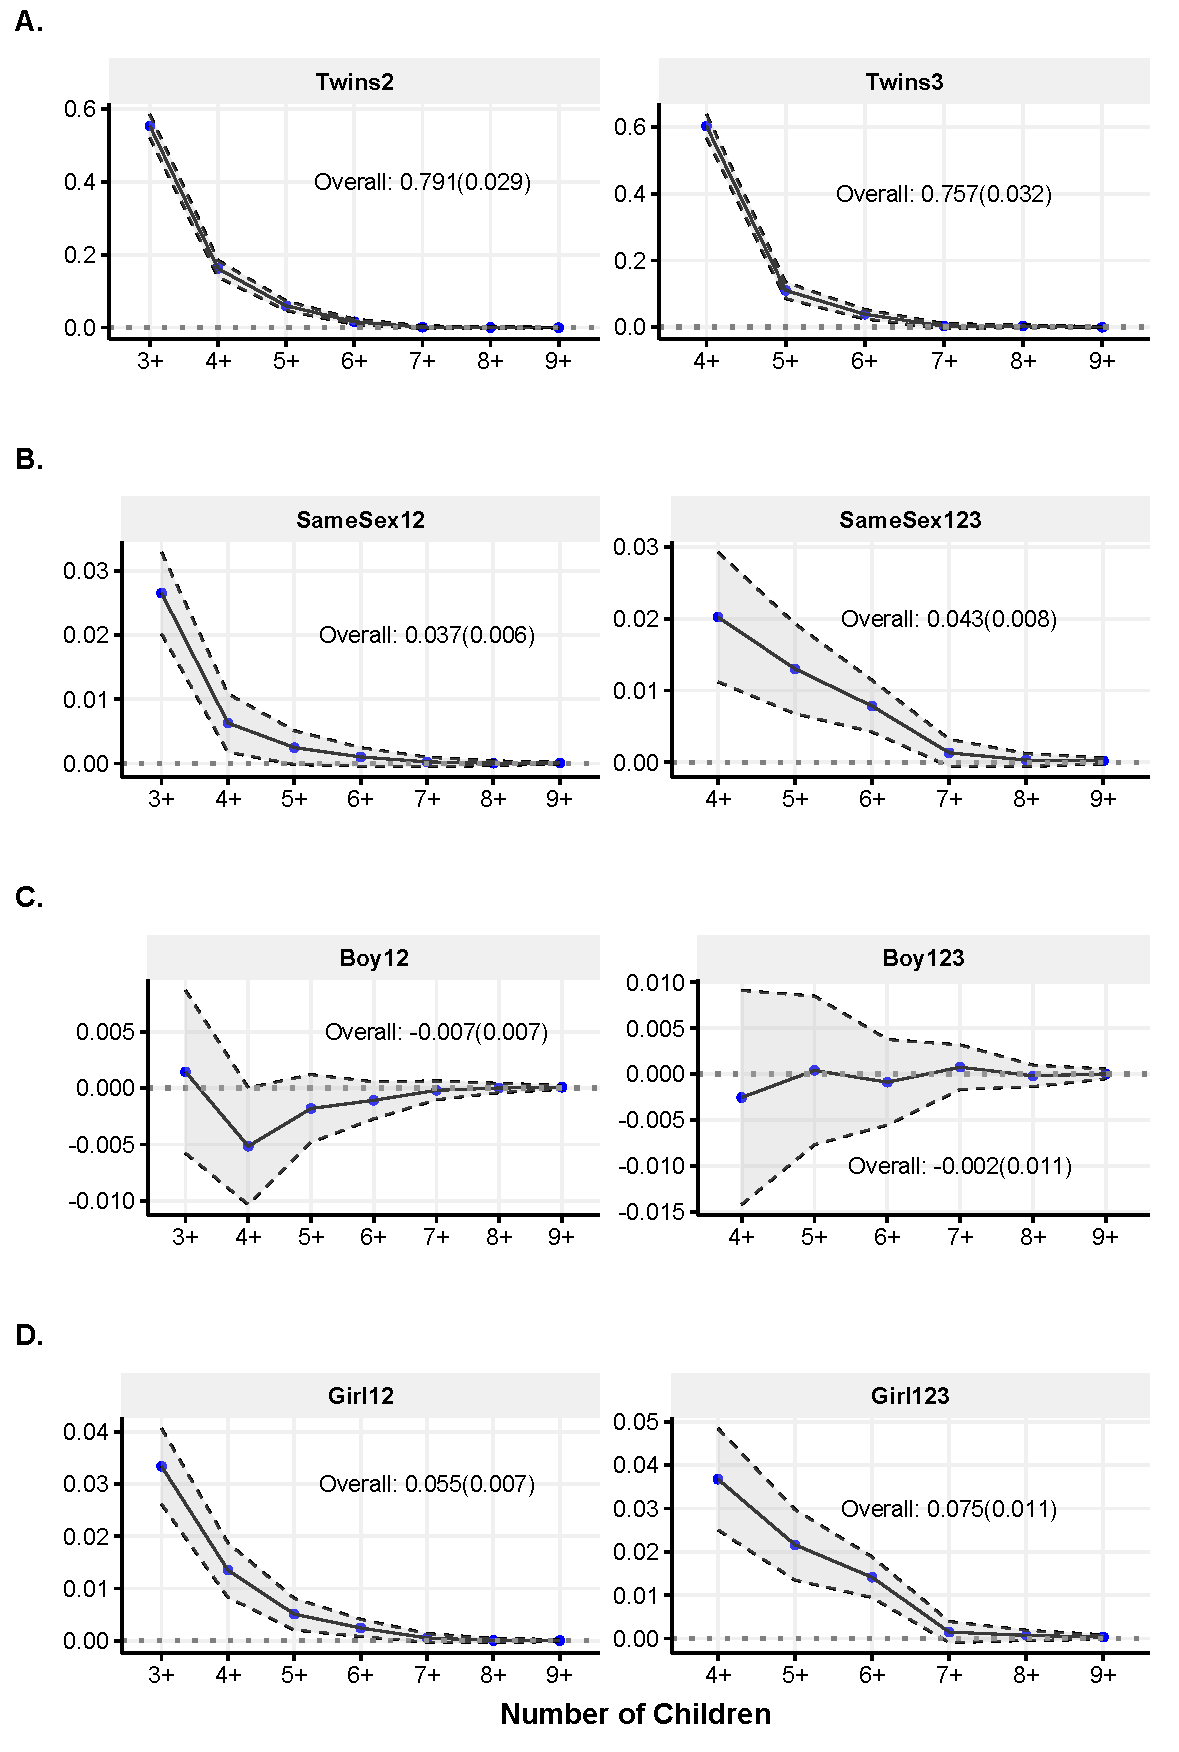
\includegraphics[width=\textwidth]{figures/acrs.pdf}
% This could go to the addendum
\end{figure}